%\documentclass[border=12pt]{standalone}
%\usepackage{tikz}
%\usetikzlibrary{arrows,positioning,shapes.geometric}
%\begin{document}


%\tikzset{every picture/.style={line width=0.75pt}} %set default line width to 0.75pt        
\begin{figure}[H]


\tikzset{every picture/.style={line width=0.75pt}} %set default line width to 0.75pt        

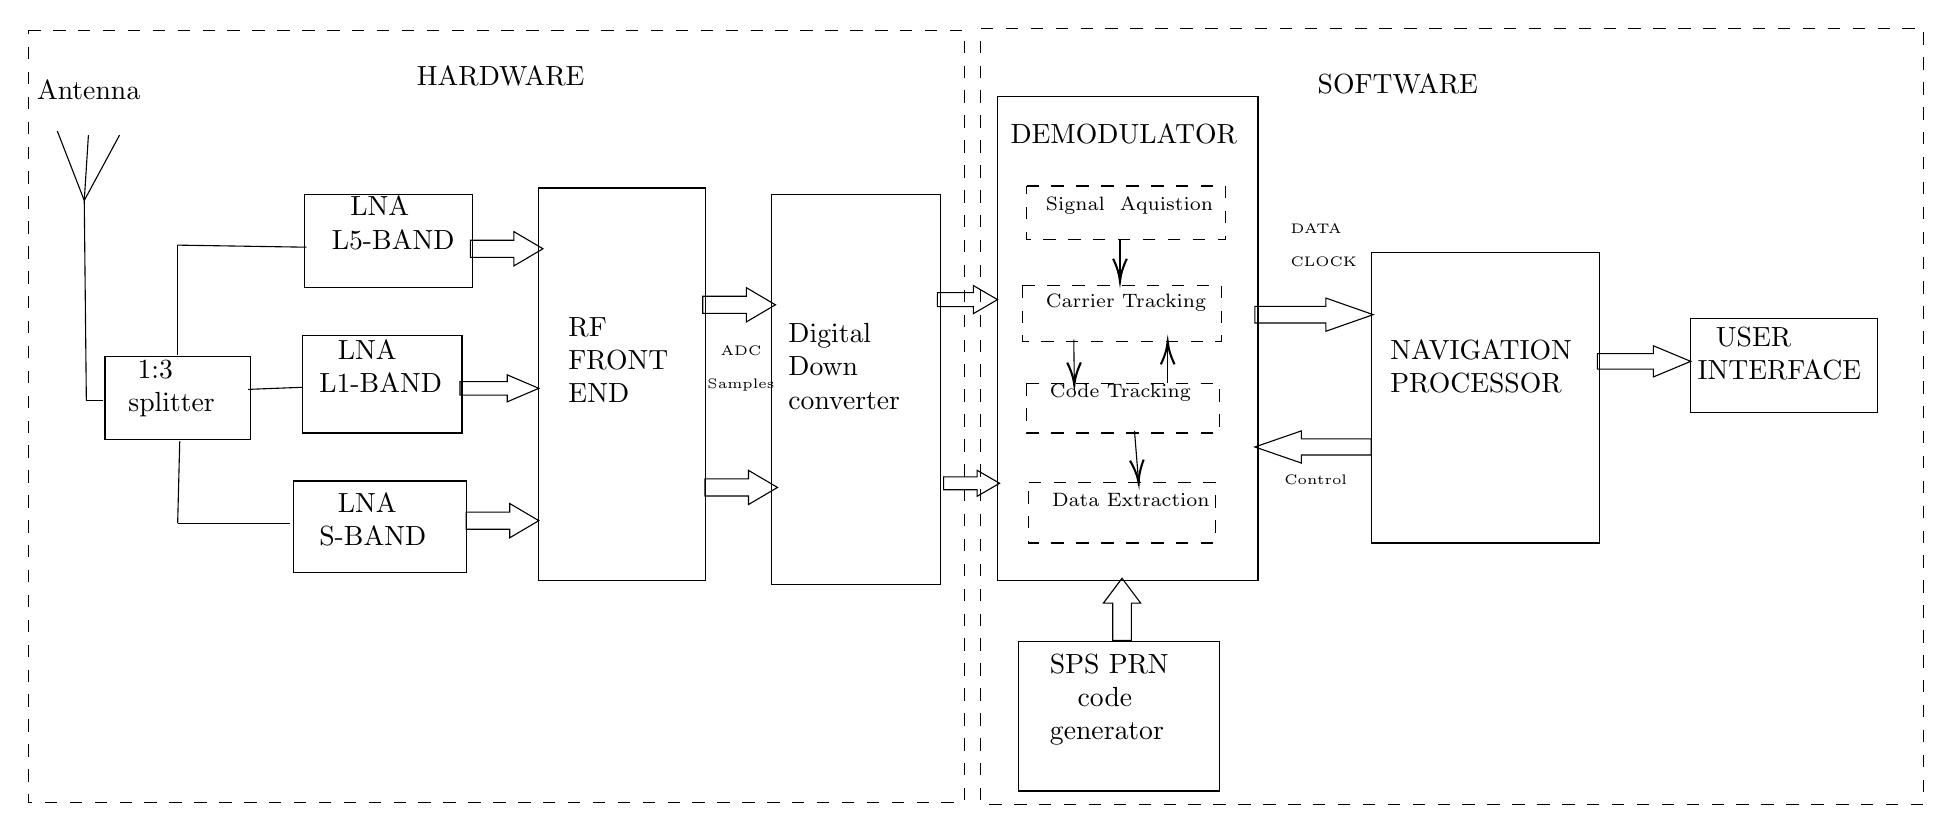
\begin{tikzpicture}[x=0.75pt,y=0.75pt,yscale=-1,xscale=1]
%uncomment if require: \path (0,418); %set diagram left start at 0, and has height of 418

%Shape: Rectangle [id:dp91775771381591] 
\draw   (38,182) -- (108,182) -- (108,222) -- (38,222) -- cycle ;
%Shape: Rectangle [id:dp6878402250141991] 
\draw   (134,104) -- (215,104) -- (215,149) -- (134,149) -- cycle ;
%Shape: Rectangle [id:dp44768197824429146] 
\draw   (129,242.13) -- (212,242.13) -- (212,286.13) -- (129,286.13) -- cycle ;
%Shape: Rectangle [id:dp5655754137730491] 
\draw   (247,101) -- (327.5,101) -- (327.5,290) -- (247,290) -- cycle ;
%Shape: Rectangle [id:dp570158544072791] 
\draw   (359,104) -- (440.5,104) -- (440.5,292) -- (359,292) -- cycle ;
%Shape: Rectangle [id:dp6780374126781124] 
\draw   (468,57) -- (593.5,57) -- (593.5,290) -- (468,290) -- cycle ;
%Shape: Rectangle [id:dp38178392589317034] 
\draw   (648,132) -- (758,132) -- (758,272) -- (648,272) -- cycle ;
%Shape: Rectangle [id:dp48587293841162293] 
\draw   (802,164) -- (892,164) -- (892,209) -- (802,209) -- cycle ;
%Shape: Rectangle [id:dp527299782431056] 
\draw  [dash pattern={on 4.5pt off 4.5pt}] (482,100) -- (578,100) -- (578,126) -- (482,126) -- cycle ;
%Shape: Rectangle [id:dp25121868516157364] 
\draw  [dash pattern={on 4.5pt off 4.5pt}] (480,148) -- (576,148) -- (576,175) -- (480,175) -- cycle ;
%Shape: Rectangle [id:dp7112717721020039] 
\draw  [dash pattern={on 4.5pt off 4.5pt}] (482,195) -- (575,195) -- (575,219) -- (482,219) -- cycle ;
%Shape: Rectangle [id:dp6802603568978252] 
\draw  [dash pattern={on 4.5pt off 4.5pt}] (483,243) -- (573,243) -- (573,272) -- (483,272) -- cycle ;
%Right Arrow [id:dp3847468665289855] 
\draw   (757,180.75) -- (784,180.75) -- (784,177) -- (802,184.5) -- (784,192) -- (784,188.25) -- (757,188.25) -- cycle ;
%Right Arrow [id:dp11379212184339593] 
\draw   (592,158) -- (626.2,158) -- (626.2,154) -- (649,162) -- (626.2,170) -- (626.2,166) -- (592,166) -- cycle ;
%Left Arrow [id:dp3964692546932914] 
\draw   (592,225.75) -- (614.4,218) -- (614.4,221.88) -- (648,221.88) -- (648,229.63) -- (614.4,229.63) -- (614.4,233.5) -- cycle ;
%Right Arrow [id:dp047248875449849015] 
\draw   (214,126.13) -- (235,126.13) -- (235,122) -- (249,130.25) -- (235,138.5) -- (235,134.38) -- (214,134.38) -- cycle ;
%Straight Lines [id:da16506188383170162] 
\draw    (28,107) -- (29,203.5) ;
%Straight Lines [id:da053092707540165485] 
\draw    (29,203.5) -- (37,203.5) ;
%Straight Lines [id:da7479103158784801] 
\draw    (15,73.5) -- (28,107) ;
%Straight Lines [id:da023170939991778106] 
\draw    (30,75.5) -- (28,107) ;
%Straight Lines [id:da6039548016175794] 
\draw    (28,107) -- (45,75.5) ;
%Straight Lines [id:da397178408511075] 
\draw    (73,128.5) -- (135,129.5) ;
%Straight Lines [id:da6398771401584881] 
\draw    (73,128.5) -- (73,181.5) ;
%Straight Lines [id:da8993427310127735] 
\draw    (74,223) -- (73,262.5) ;
%Straight Lines [id:da5504549537888844] 
\draw    (73,262.5) -- (127,262.5) ;
%Right Arrow [id:dp38901755194750065] 
\draw   (212,257.13) -- (233,257.13) -- (233,253) -- (247,261.25) -- (233,269.5) -- (233,265.38) -- (212,265.38) -- cycle ;
%Right Arrow [id:dp9617272144769732] 
\draw   (326,153.13) -- (347,153.13) -- (347,149) -- (361,157.25) -- (347,165.5) -- (347,161.38) -- (326,161.38) -- cycle ;
%Right Arrow [id:dp24676205787927274] 
\draw   (327,241.13) -- (348,241.13) -- (348,237) -- (362,245.25) -- (348,253.5) -- (348,249.38) -- (327,249.38) -- cycle ;
%Right Arrow [id:dp7057810479841495] 
\draw   (439,151.38) -- (456.4,151.38) -- (456.4,148) -- (468,154.75) -- (456.4,161.5) -- (456.4,158.13) -- (439,158.13) -- cycle ;
%Right Arrow [id:dp5533926878537673] 
\draw   (442,240.13) -- (458.2,240.13) -- (458.2,237) -- (469,243.25) -- (458.2,249.5) -- (458.2,246.38) -- (442,246.38) -- cycle ;
%Shape: Rectangle [id:dp6070084344522547] 
\draw   (478,319.5) -- (575,319.5) -- (575,391.5) -- (478,391.5) -- cycle ;
%Up Arrow [id:dp35040919221179934] 
\draw   (519,301) -- (528,289) -- (537,301) -- (532.5,301) -- (532.5,319) -- (523.5,319) -- (523.5,301) -- cycle ;
%Shape: Rectangle [id:dp11970499763022935] 
\draw   (133,172) -- (210,172) -- (210,219) -- (133,219) -- cycle ;
%Right Arrow [id:dp9092739703716787] 
\draw   (209,194.25) -- (231.8,194.25) -- (231.8,191) -- (247,197.5) -- (231.8,204) -- (231.8,200.75) -- (209,200.75) -- cycle ;
%Straight Lines [id:da37176764113278415] 
\draw    (107,198) -- (133,197) ;
%Shape: Rectangle [id:dp7313088111701439] 
\draw  [dash pattern={on 4.5pt off 4.5pt}] (1,25) -- (452,25) -- (452,397) -- (1,397) -- cycle ;
%Shape: Rectangle [id:dp7087849934206134] 
\draw  [dash pattern={on 4.5pt off 4.5pt}] (460,24) -- (914,24) -- (914,398) -- (460,398) -- cycle ;
%Straight Lines [id:da9288054715368911] 
\draw    (527,126) -- (527,144) ;
\draw [shift={(527,146)}, rotate = 270] [color={rgb, 255:red, 0; green, 0; blue, 0 }  ][line width=0.75]    (10.93,-3.29) .. controls (6.95,-1.4) and (3.31,-0.3) .. (0,0) .. controls (3.31,0.3) and (6.95,1.4) .. (10.93,3.29)   ;
%Straight Lines [id:da919835721260752] 
\draw    (504.75,174) -- (504.98,194) ;
\draw [shift={(505,196)}, rotate = 269.35] [color={rgb, 255:red, 0; green, 0; blue, 0 }  ][line width=0.75]    (10.93,-3.29) .. controls (6.95,-1.4) and (3.31,-0.3) .. (0,0) .. controls (3.31,0.3) and (6.95,1.4) .. (10.93,3.29)   ;
%Straight Lines [id:da9561713820062974] 
\draw    (550,195) -- (550,177) ;
\draw [shift={(550,175)}, rotate = 90] [color={rgb, 255:red, 0; green, 0; blue, 0 }  ][line width=0.75]    (10.93,-3.29) .. controls (6.95,-1.4) and (3.31,-0.3) .. (0,0) .. controls (3.31,0.3) and (6.95,1.4) .. (10.93,3.29)   ;
%Straight Lines [id:da27644261005727155] 
\draw    (534,218) -- (534.38,222.81) -- (535.84,241.01) ;
\draw [shift={(536,243)}, rotate = 265.43] [color={rgb, 255:red, 0; green, 0; blue, 0 }  ][line width=0.75]    (10.93,-3.29) .. controls (6.95,-1.4) and (3.31,-0.3) .. (0,0) .. controls (3.31,0.3) and (6.95,1.4) .. (10.93,3.29)   ;

% Text Node
\draw (490,104) node [anchor=north west][inner sep=0.75pt]   [align=left] {{\scriptsize Signal \ Aquistion }};
% Text Node
\draw (490,151) node [anchor=north west][inner sep=0.75pt]   [align=left] {{\scriptsize Carrier Tracking}};
% Text Node
\draw (492,194) node [anchor=north west][inner sep=0.75pt]   [align=left] {{\scriptsize Code Tracking }};
% Text Node
\draw (493,247) node [anchor=north west][inner sep=0.75pt]   [align=left] {{\scriptsize Data Extraction}};
% Text Node
\draw (473,69) node [anchor=north west][inner sep=0.75pt]   [align=left] {DEMODULATOR};
% Text Node
\draw (656,173) node [anchor=north west][inner sep=0.75pt]   [align=left] {NAVIGATION\\PROCESSOR};
% Text Node
\draw (804,167) node [anchor=north west][inner sep=0.75pt]   [align=left] { \ \ USER\\INTERFACE};
% Text Node
\draw (608,117) node [anchor=north west][inner sep=0.75pt]   [align=left] {{\tiny DATA }\\{\tiny CLOCK}};
% Text Node
\draw (605,238) node [anchor=north west][inner sep=0.75pt]   [align=left] {{\tiny Control}};
% Text Node
\draw (366,165) node [anchor=north west][inner sep=0.75pt]   [align=left] {Digital\\Down\\converter \\};
% Text Node
\draw (260,162) node [anchor=north west][inner sep=0.75pt]   [align=left] {RF\\FRONT \\END};
% Text Node
\draw (140,247) node [anchor=north west][inner sep=0.75pt]   [align=left] { \ \ LNA \\S-BAND};
% Text Node
\draw (146,104) node [anchor=north west][inner sep=0.75pt]   [align=left] { \ \ LNA\\L5-BAND};
% Text Node
\draw (48,183) node [anchor=north west][inner sep=0.75pt]   [align=left] { \ 1:3\\splitter};
% Text Node
\draw (327,176) node [anchor=north west][inner sep=0.75pt]   [align=left] {{\tiny  \ \ ADC}\\{\tiny Samples}};
% Text Node
\draw (4,48) node [anchor=north west][inner sep=0.75pt]   [align=left] {Antenna};
% Text Node
\draw (492,324.5) node [anchor=north west][inner sep=0.75pt]   [align=left] {SPS PRN \\ \ \ \ code \\generator};
% Text Node
\draw (140,173) node [anchor=north west][inner sep=0.75pt]   [align=left] { \ \ LNA\\L1-BAND};
% Text Node
\draw (187,41) node [anchor=north west][inner sep=0.75pt]   [align=left] {HARDWARE};
% Text Node
\draw (621,45) node [anchor=north west][inner sep=0.75pt]   [align=left] {SOFTWARE};


\end{tikzpicture}

\begin{figure}
%\end{document}
